%----------------------------------------------------------------------------------------
%	PROBLEM 1
%----------------------------------------------------------------------------------------

% To have just one problem per page, simply put a \clearpage after each problem
\newpage
\begin{homeworkProblem}
\section{Iterative improvement algorithms}
\subsection{Problem statement}
Implement iterative improvement algorithms with:
\begin{itemize}
  \item first-improvement
  \item best-improvement
\end{itemize}
pivoting rule for each of the three neighborhoods: transpose, exchange, and insert. \\
As a starting solution for iterative improvement, consider a random permutation, that is, use the method “Uninformed Random Picking” (see slides of lectures). Bonus points will be awarded for also considering an insertion heuristic as an alternative to random initialization.
\begin{enumerate}
  \item Run the 6 resulting iterative improvement algorithms (all combinations of the two pivoting rules and the
three neighborhoods) on each of the instances. Repeat each run 100 times with different seed for the random
number generator.
\item Compute the following statistics for each of the 6 iterative improvement algorithms and each instance:
\begin{itemize}
  \item Percentage of runs with constraint violations
  \item Mean penalised relative percentage deviation
  \item Mean computation time
\end{itemize} 
\item Produce boxplots of penalised relative percentage deviation and computation time per instance.
\item Determine using statistical tests (in this case, the Wilcoxon test), whether there is a statistically significant difference between the quality of the solutions generated by the different algorithms.
In particular, compare best vs. first-improvement for each neighborhood, and exchange vs. insertion for each pivoting rule.
\end{enumerate}

\subsection{Metric definitions}\label{subsec:metric}
For each algorithm $k$, applied on instance $i$, using different randomly generated seeds one have to compute:
\begin{itemize}
  \item Number of constraint violations
  \item Penalised relative percentage deviation (PRPD)
  \item Computation time (CPU time)
\end{itemize}

In order to perform a statistical analysis of the results, each algorithm $k$ is launched 100 times on the same instance, computing the
following statistics:
\begin{itemize}
  \item Percentage of infeasible solutions (0.x has to be interpreted as x\%) 
  \item Average Penalised relative percentage deviation.
  \item Average Computation time (CPU time).
\end{itemize}

For each instance $i$, the distributions of PRPD and Cpu Times are displayed using box plots and the Wilcoxon signed rank test is performed, in order to assess the existence of a statistically significant difference among the results obtained by the different algorithms on the same instance. 

\paragraph{Constraint Violations}
In the standard formulation of the TSP problem, a solution to the problem is represented by a permutation of the different
entities (solution components), that the hypothetical travelling salesman has to visit.

The best solution for the problem is the permutation that minimizes the total travelling time (distance) among the cities.
The presence of time windows introduce an additional constraint on the feasibility of the solution.

In fact, each solution component has an associated time window within which it has to be visited in order to guarantee the feasiblity of the tour.

Arriving in a (city) before the opening of the corresponding time window involves a delay in the total travelling time (to wait for the time window to open) whereas the arrival after the closure of the time windows will generate a constraint violation.

Thus, a solution is feasible if and only if all the time windows constraints are met, or in other words, if there are no constraint violations.

In this case, the best solution is the feasible solution which minimizes the total travel time.

\paragraph{Penalised Relative Percentage Deviation}
The penalised relative percentage deviation (PRDP from now on) is a measure of the solution quality, with respect to the best known
solution for the instance, taking into account a strong penalisation for the violation of constraints.
The PRPD is computed as follows:
\begin{equation}
pRPD_{kri} = 100 \cdot \frac{(f_{kri} + 10^4\cdot\Omega_{kri})-best_i}{best_i}
\end{equation}

\paragraph{Runtime}
The runtime is a measure of both the quality and the time complexity of the algorithm.

It is measured using the function \verb|int clock_gettime(clockid_t clk_id, struct timespect *tp)| from the \verb|time.h| library.

The parameter \verb|clk_id=CLOCK_PROCESS_CPUTIME_ID|, is used to read the values from an high-resolution timer provided by the CPU for each process.

The runtime is computed (using the user defined function \verb|ComputeRunTime|) as the difference, with a resolution of $10^-9$ s, from the time obtained using \verb|clock_gettime| at the beginning and the one obtained at the end of the simulation.

\subsection{Experiment results}
\subsubsection{n80w20.001}
\begin{center}
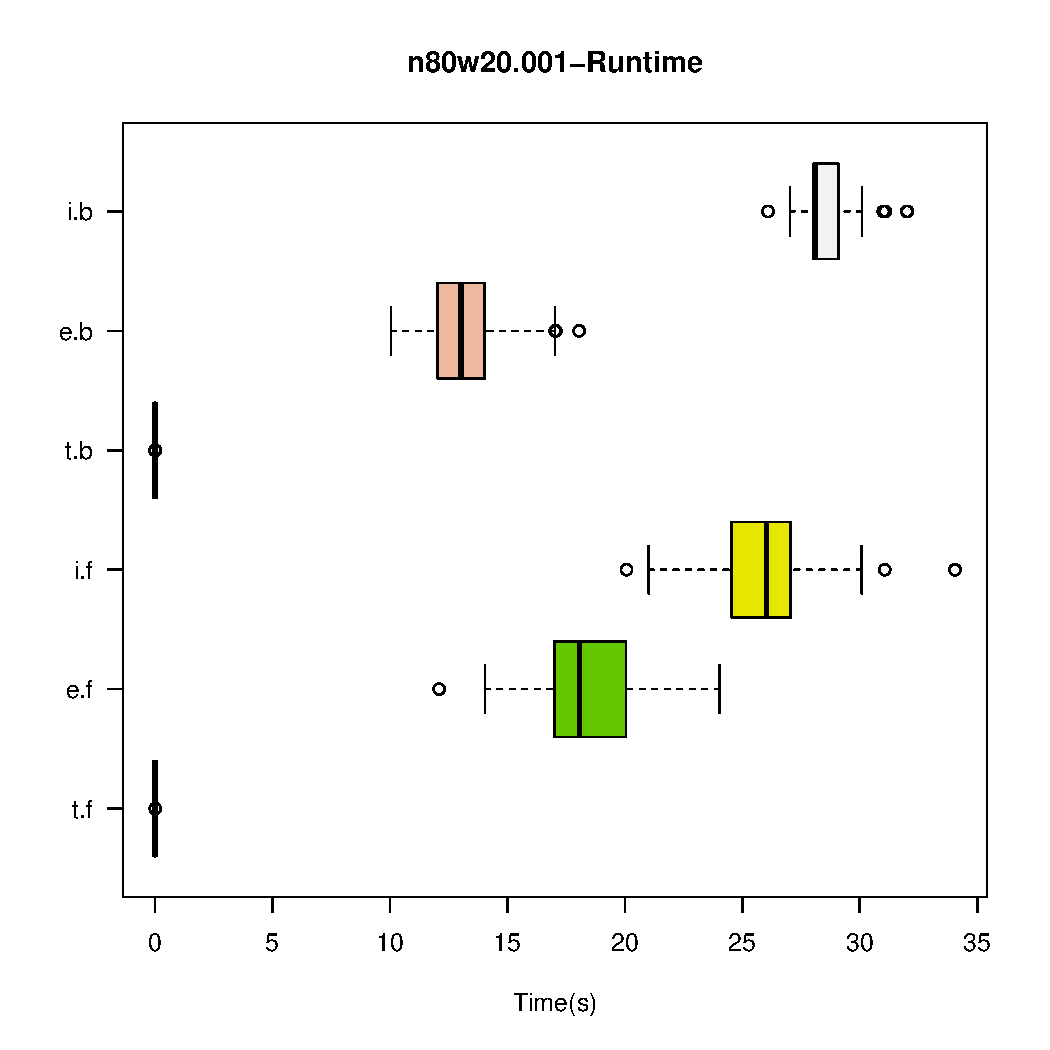
\includegraphics[width=0.6\textwidth,keepaspectratio]{{II/n80w20.001/n80w20.001-CpuTime}.pdf}
\captionof{figure}{n80w20.001 - Runtime boxplots for the different iterative improvement algorithms}
\end{center}

\begin{center}
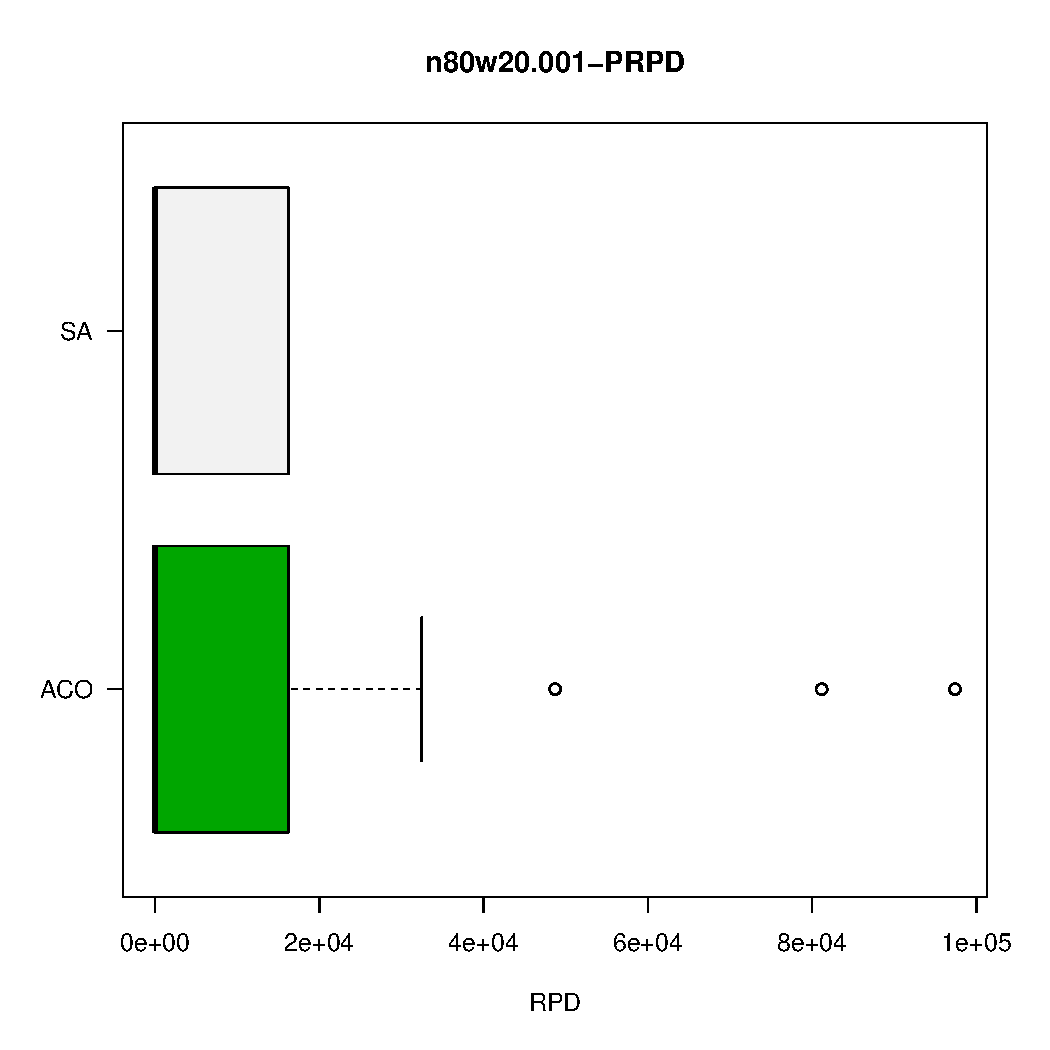
\includegraphics[width=0.6\textwidth,keepaspectratio]{{II/n80w20.001/n80w20.001-PRPD}.pdf}
\captionof{figure}{n80w20.001 - PRPD boxplots for the different iterative improvement algorithms}
\end{center}

\begin{center}
\begin{tabular}{|l|l|}
\hline
\textbf{Test} & \textbf{P-Value} \\
\hline
First vs best - Transpose&9.74631639820544e-18\\
\hline
First vs best - Exchange&2.04966732989559e-17\\
\hline
First vs best - Insert&1.74838327736385e-15\\
\hline
Exchange vs Insert - First&3.95591160889952e-18\\
\hline
Exchange vs Insert - Best&3.9556885406462e-18\\
\hline
\end{tabular}
\captionof{table}{n80w20.001 - Results of Wilcoxon paired signed rank test}
\label{tab:w.1}
\end{center}

\subsubsection{n80w20.002}
\begin{center}
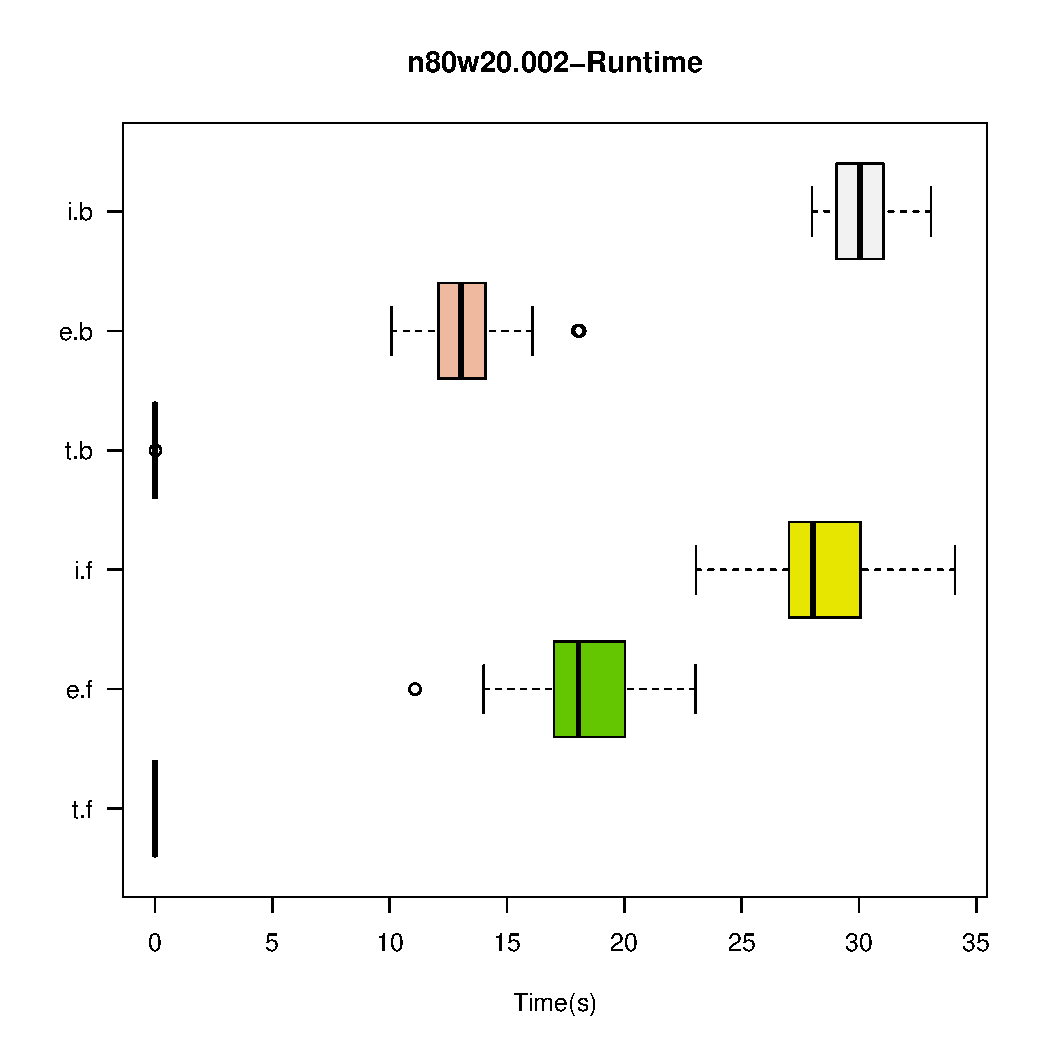
\includegraphics[width=0.6\textwidth,keepaspectratio]{{II/n80w20.002/n80w20.002-CpuTime}.pdf}
\captionof{figure}{n80w20.002 - Runtime boxplots for the different iterative improvement algorithms}
\end{center}

\begin{center}
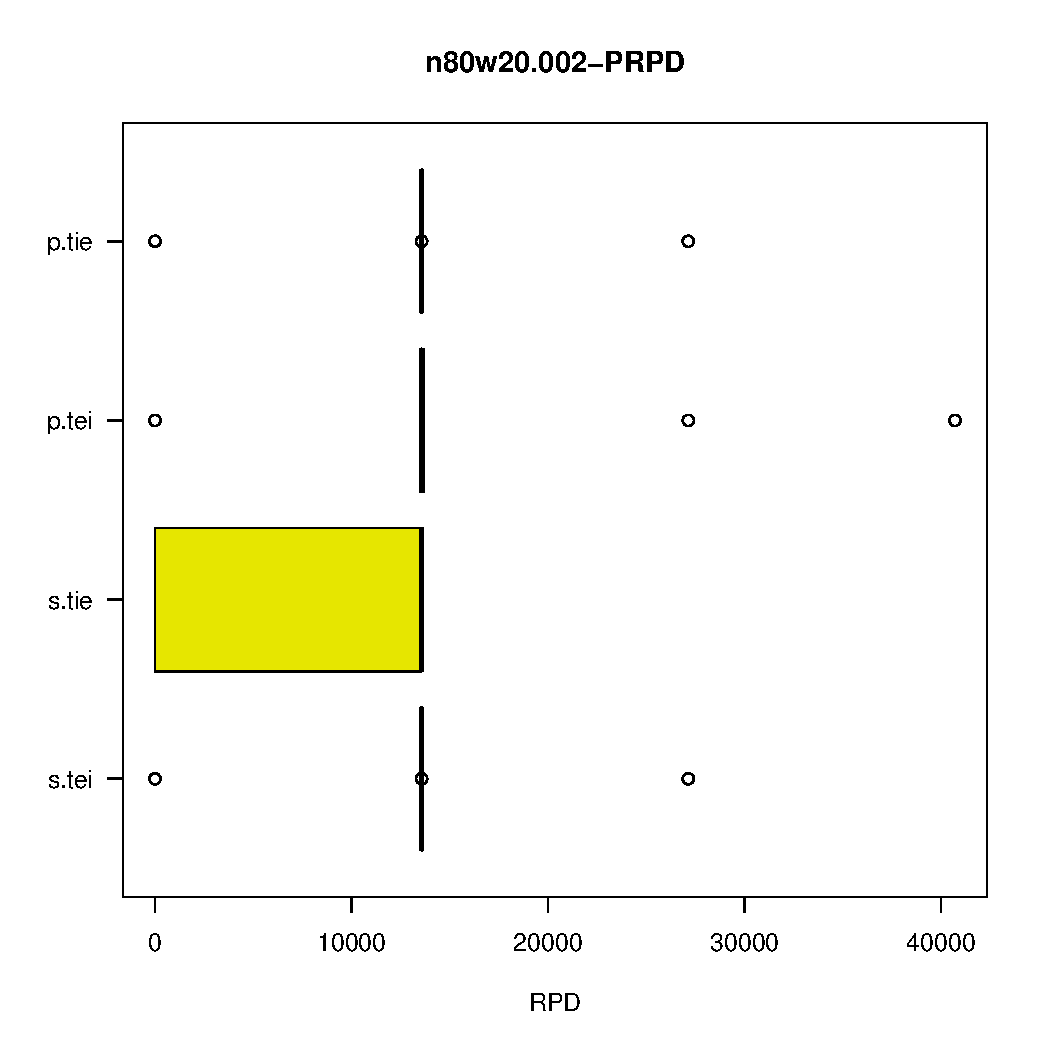
\includegraphics[width=0.6\textwidth,keepaspectratio]{{II/n80w20.002/n80w20.002-PRPD}.pdf}
\captionof{figure}{n80w20.002 - PRPD boxplots for the different iterative improvement algorithms}
\end{center}

\begin{center}
\begin{tabular}{|l|l|}
\hline
\textbf{Test} & \textbf{P-Value} \\
\hline
First vs best - Transpose&3.95591160889952e-18\\
\hline
First vs best - Exchange&1.61703099974578e-17\\
\hline
First vs best - Insert&2.39050570998277e-07\\
\hline
Exchange vs Insert - First&3.95591160889952e-18\\
\hline
Exchange vs Insert - Best&3.9556885406462e-18\\
\hline
\end{tabular}
\captionof{table}{n80w20.002 - Results of Wilcoxon paired signed rank test}
\label{tab:w.2}
\end{center}

\subsubsection{n80w20.003}
\begin{center}
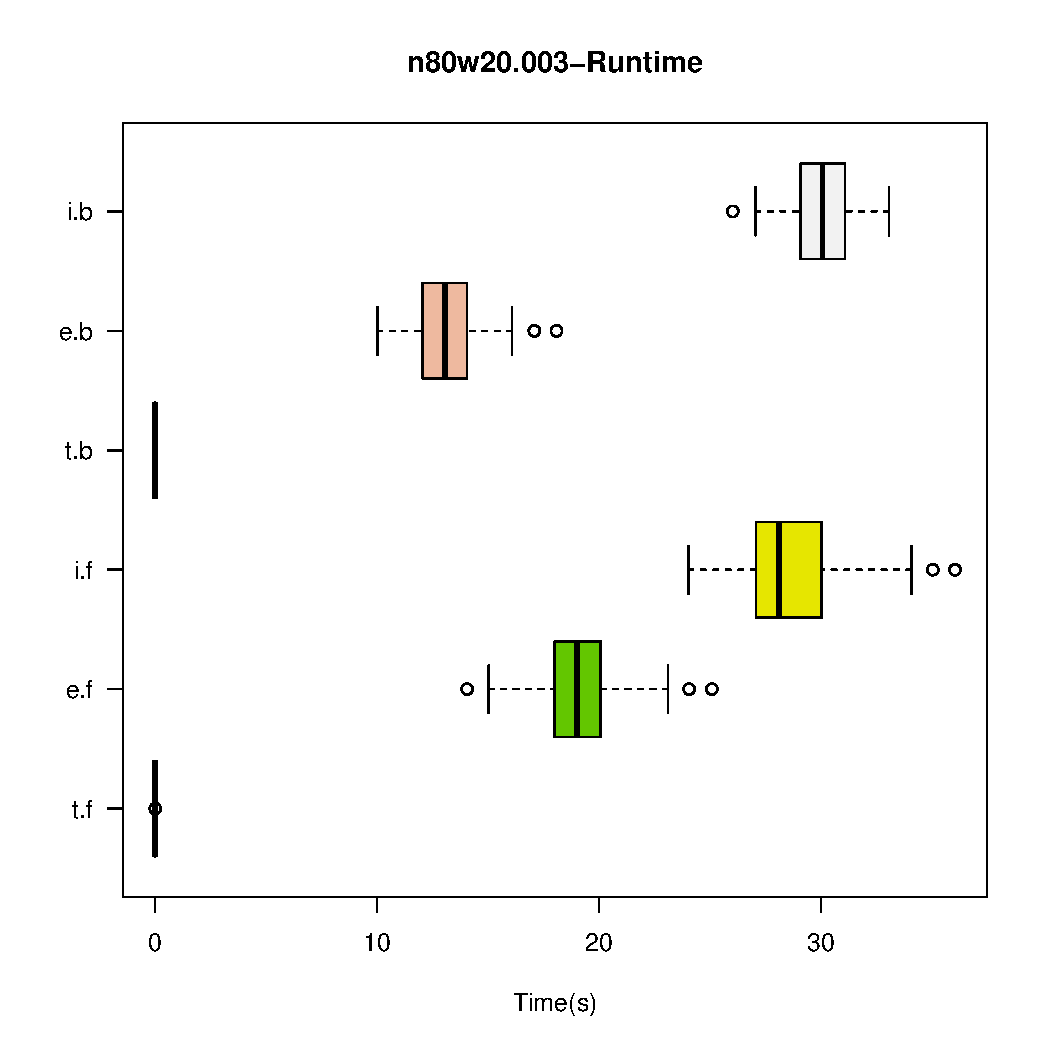
\includegraphics[width=0.6\textwidth,keepaspectratio]{{II/n80w20.003/n80w20.003-CpuTime}.pdf}
\captionof{figure}{n80w20.003 - Runtime boxplots for the different iterative improvement algorithms}
\end{center}

\begin{center}
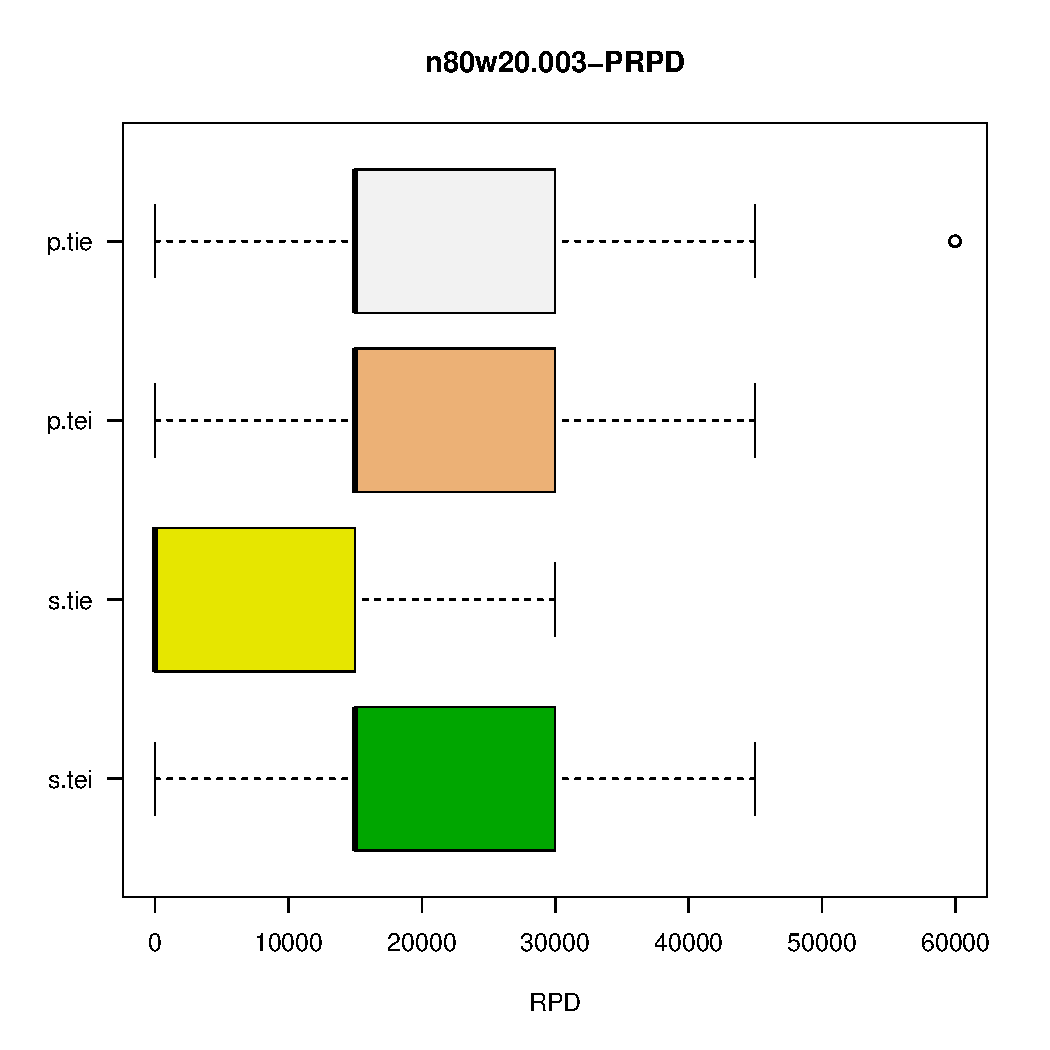
\includegraphics[width=0.6\textwidth,keepaspectratio]{{II/n80w20.003/n80w20.003-PRPD}.pdf}
\captionof{figure}{n80w20.003 - PRPD boxplots for the different iterative improvement algorithms}
\end{center}

\begin{center}
\begin{tabular}{|l|l|}
\hline
\textbf{Test} & \textbf{P-Value} \\
\hline
First vs best - Transpose&3.95591160889952e-18\\
\hline
First vs best - Exchange&6.21747363653032e-18\\
\hline
First vs best - Insert&6.2952945764779e-08\\
\hline
Exchange vs Insert - First&3.9556885406462e-18\\
\hline
Exchange vs Insert - Best&3.95591160889952e-18\\
\hline
\end{tabular}
\captionof{table}{n80w20.003 - Results of Wilcoxon paired signed rank test}
\label{tab:w.3}
\end{center}

\subsubsection{n80w20.004}
\begin{center}
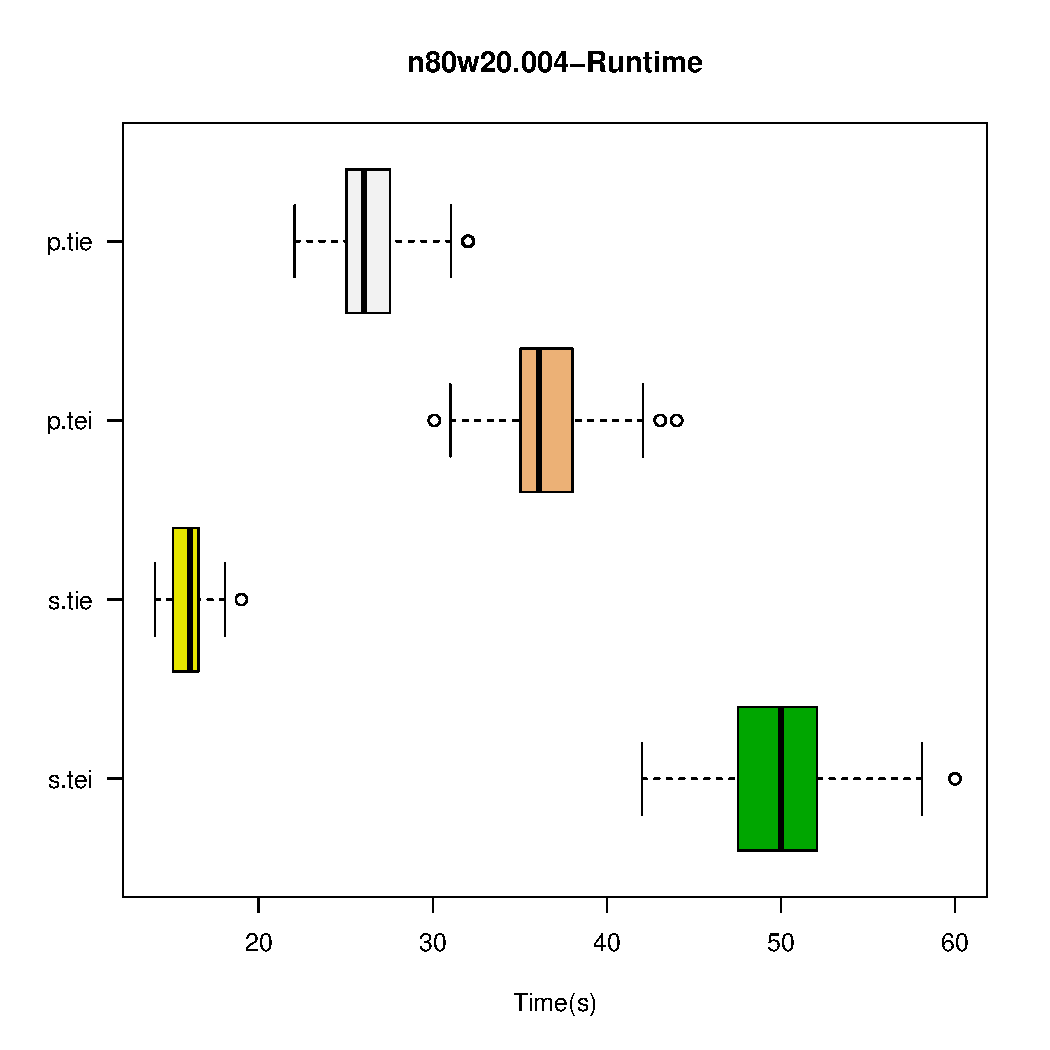
\includegraphics[width=0.6\textwidth,keepaspectratio]{{II/n80w20.004/n80w20.004-CpuTime}.pdf}
\captionof{figure}{n80w20.004 - Runtime boxplots for the different iterative improvement algorithms}
\end{center}

\begin{center}
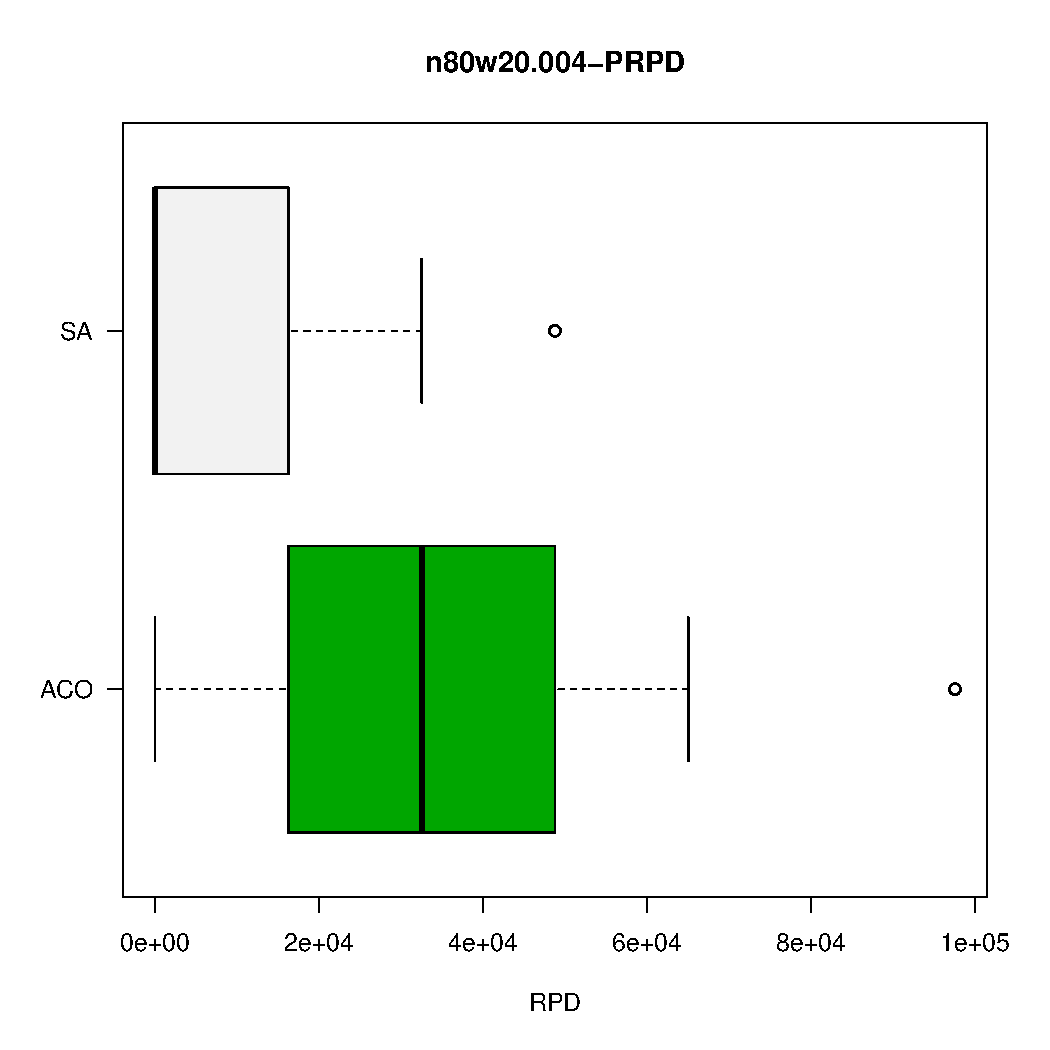
\includegraphics[width=0.6\textwidth,keepaspectratio]{{II/n80w20.004/n80w20.004-PRPD}.pdf}
\captionof{figure}{n80w20.001 - PRPD boxplots for the different iterative improvement algorithms}
\end{center}

\begin{center}
\begin{tabular}{|l|l|}
\hline
\textbf{Test} & \textbf{P-Value} \\
\hline
First vs best - Transpose&4.33123080260219e-18\\
\hline
First vs best - Exchange&1.5356610755813e-16\\
\hline
First vs best - Insert&4.27702026764362e-14\\
\hline
Exchange vs Insert - First&5.59593516960623e-18\\
\hline
Exchange vs Insert - Best&3.95591160889952e-18\\
\hline
\end{tabular}
\captionof{table}{n80w20.004 - Results of Wilcoxon paired signed rank test}
\label{tab:w.4}
\end{center}

\subsubsection{n80w20.005}
\begin{center}
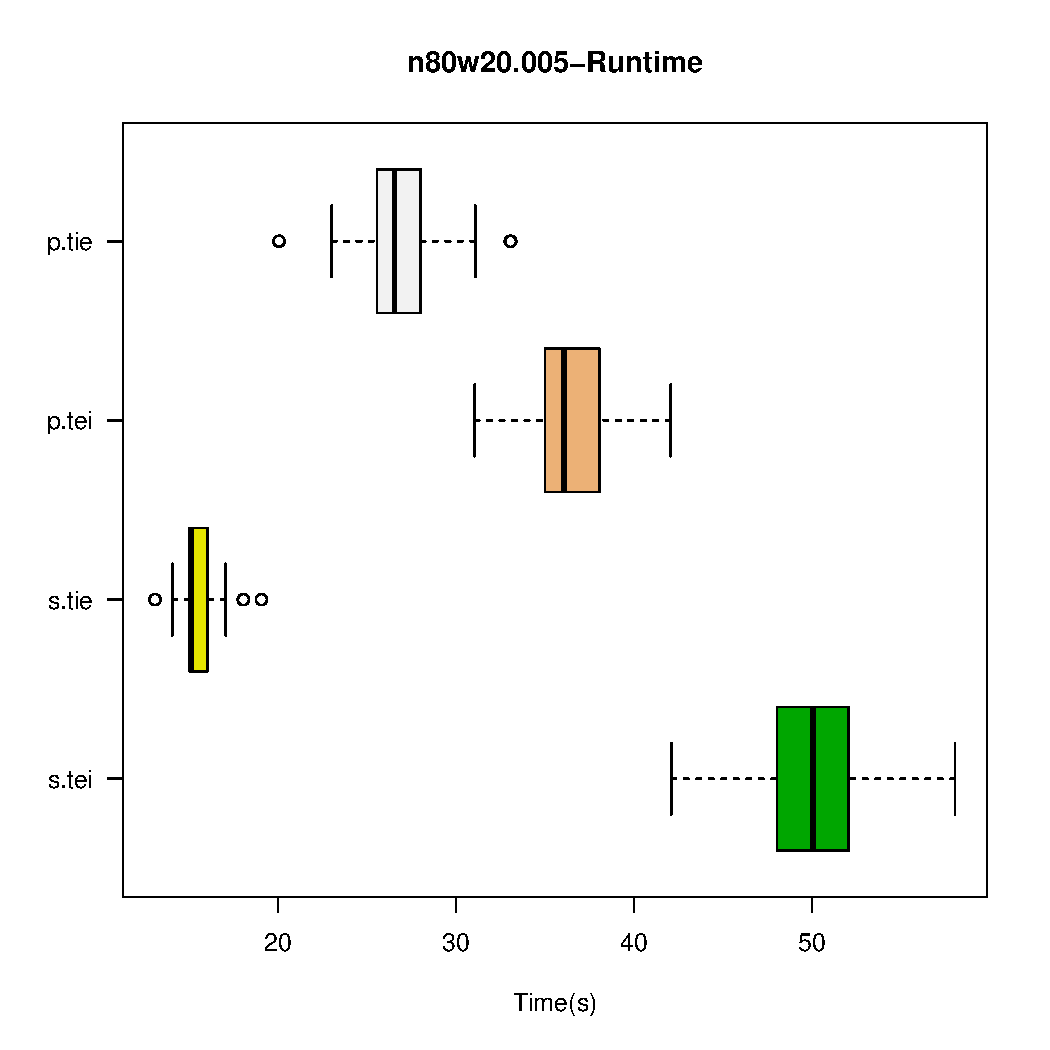
\includegraphics[width=0.6\textwidth,keepaspectratio]{{II/n80w20.005/n80w20.005-CpuTime}.pdf}
\captionof{figure}{n80w20.005 - Runtime boxplots for the different iterative improvement algorithms}
\end{center}

\begin{center}
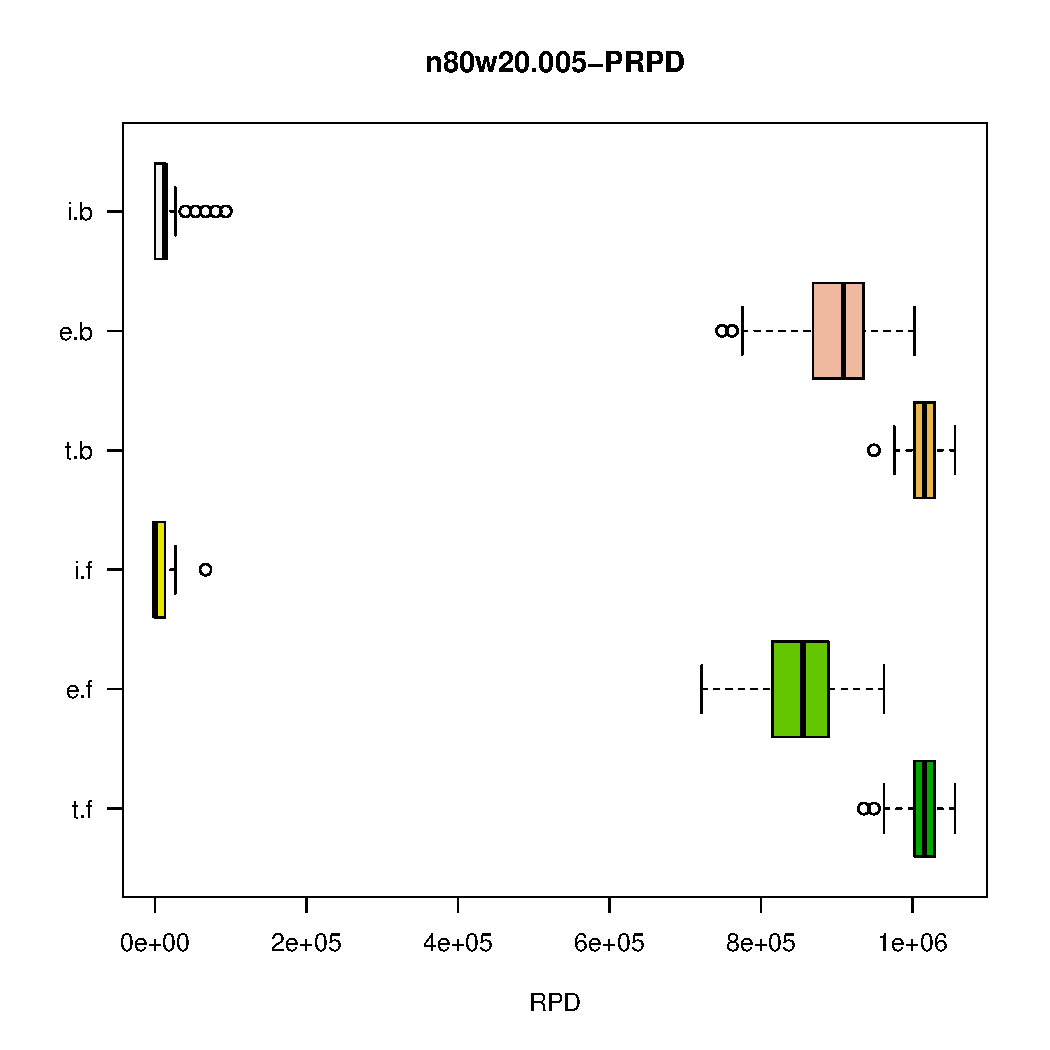
\includegraphics[width=0.6\textwidth,keepaspectratio]{{II/n80w20.005/n80w20.005-PRPD}.pdf}
\captionof{figure}{n80w20.005 - PRPD boxplots for the different iterative improvement algorithms}
\end{center}

\begin{center}
\begin{tabular}{|l|l|}
\hline
\textbf{Test} & \textbf{P-Value} \\
\hline
First vs best - Transpose&4.46398542390809e-18\\
\hline
First vs best - Exchange&4.74166029806301e-18\\
\hline
First vs best - Insert&4.0369131744045e-10\\
\hline
Exchange vs Insert - First&4.74166029806301e-18\\
\hline
Exchange vs Insert - Best&3.95591160889952e-18\\
\hline
\end{tabular}
\captionof{table}{n80w20.005 - Results of Wilcoxon paired signed rank test}
\label{tab:w.5}
\end{center}

\subsubsection{n80w200.001}
\begin{center}
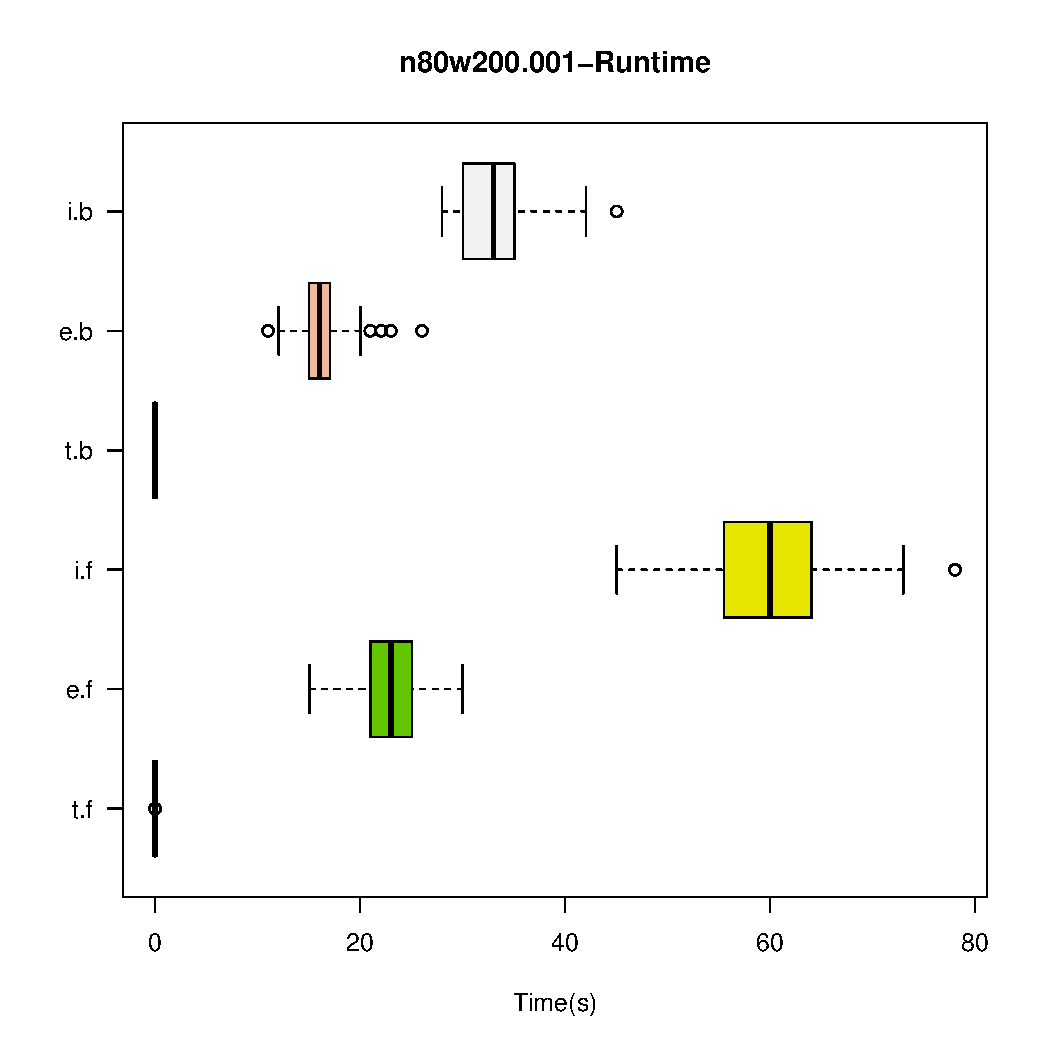
\includegraphics[width=0.6\textwidth,keepaspectratio]{{II/n80w200.001/n80w200.001-CpuTime}.pdf}
\captionof{figure}{n80w200.001 - Runtime boxplots for the different iterative improvement algorithms}
\end{center}

\begin{center}
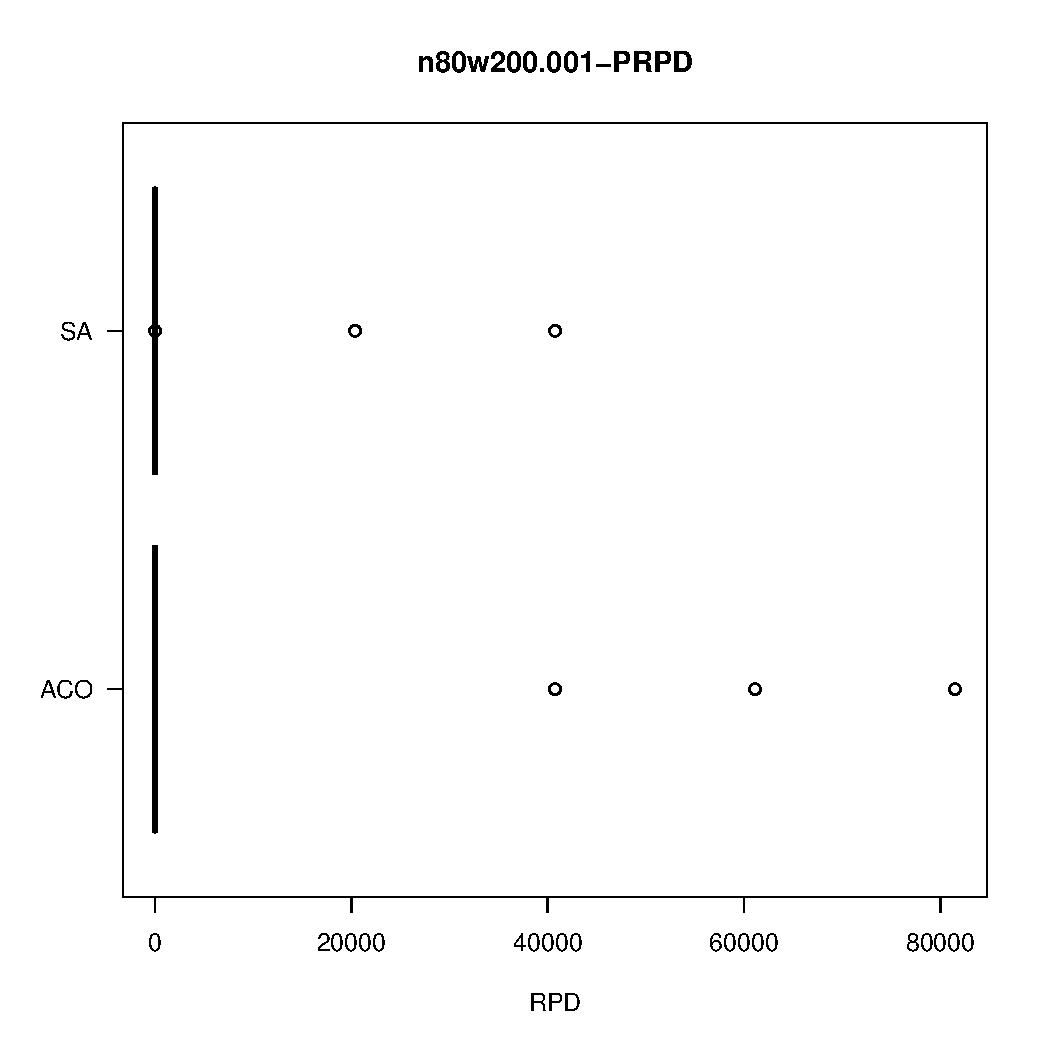
\includegraphics[width=0.6\textwidth,keepaspectratio]{{II/n80w200.001/n80w200.001-PRPD}.pdf}
\captionof{figure}{n80w200.001 - PRPD boxplots for the different iterative improvement algorithms}
\end{center}

\begin{center}
\begin{tabular}{|l|l|}
\hline
\textbf{Test} & \textbf{P-Value} \\
\hline
First vs best - Transpose&4.07730530936212e-18\\
\hline
First vs best - Exchange&2.17457280454137e-17\\
\hline
First vs best - Insert&3.95591160889952e-18\\
\hline
Exchange vs Insert - First&3.95591160889952e-18\\
\hline
Exchange vs Insert - Best&3.95591160889952e-18\\
\hline
\end{tabular}
\captionof{table}{n80w200.001 - Results of Wilcoxon paired signed rank test}
\label{tab:w.6}
\end{center}

\subsubsection{n80w200.002}
\begin{center}
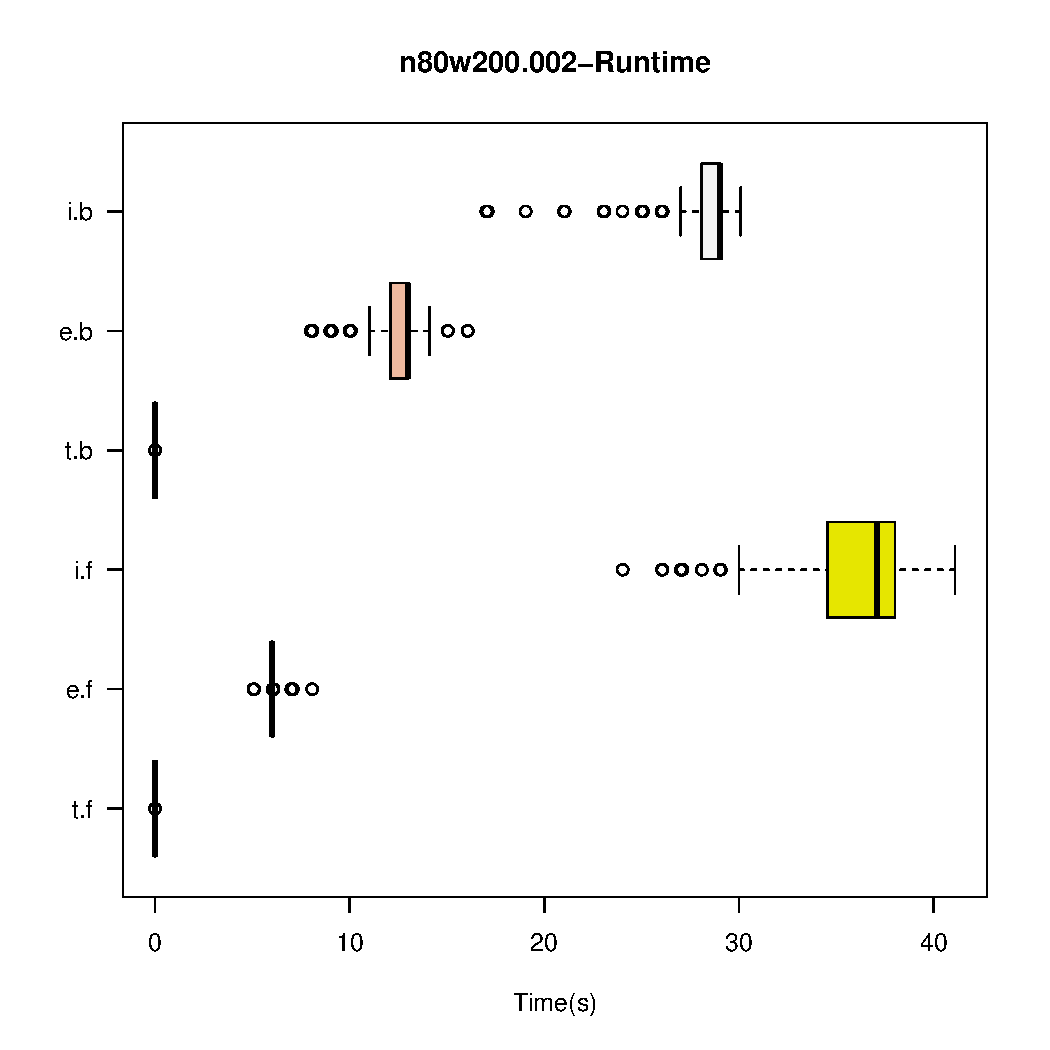
\includegraphics[width=0.6\textwidth,keepaspectratio]{{II/n80w200.002/n80w200.002-CpuTime}.pdf}
\captionof{figure}{n80w200.002 - Runtime boxplots for the different iterative improvement algorithms}
\end{center}

\begin{center}
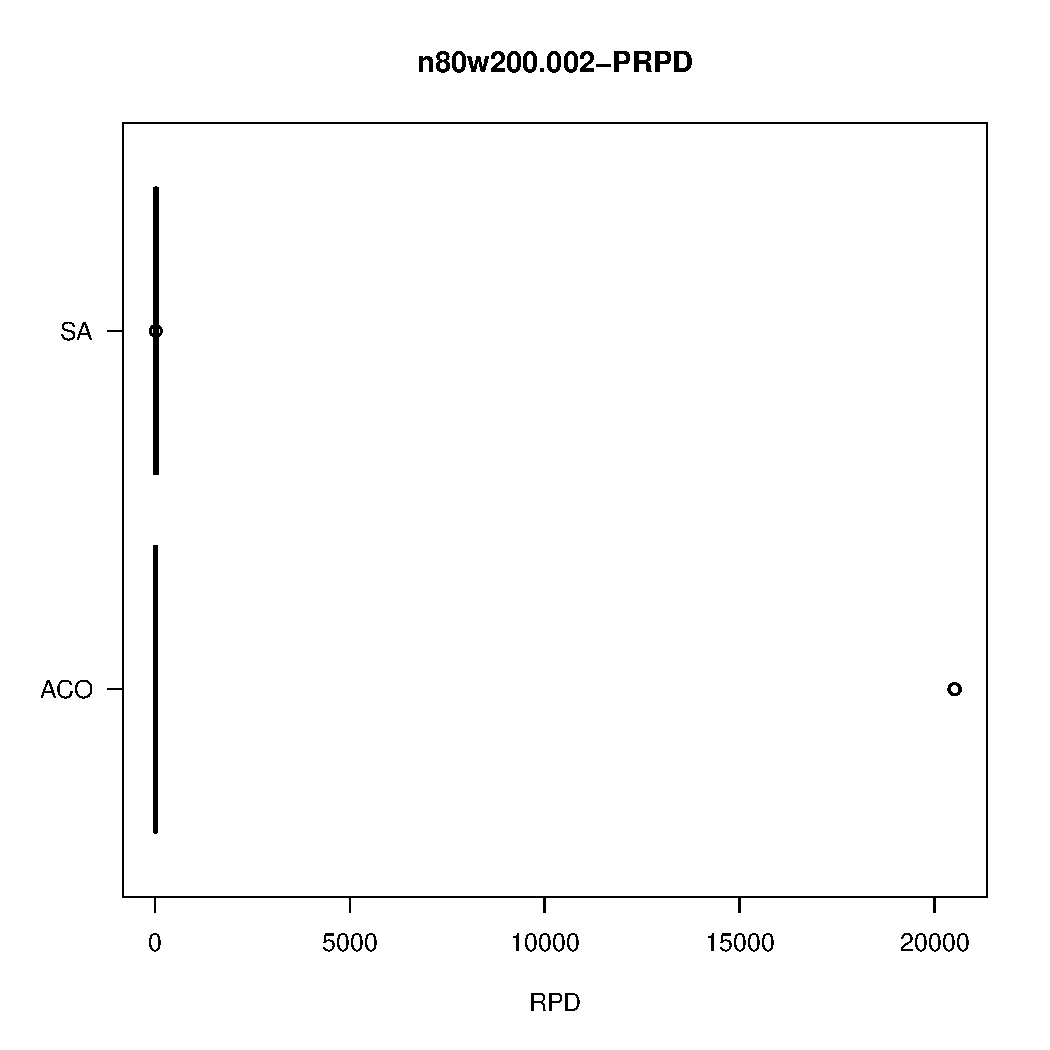
\includegraphics[width=0.6\textwidth,keepaspectratio]{{II/n80w200.002/n80w200.002-PRPD}.pdf}
\captionof{figure}{n80w200.002 - PRPD boxplots for the different iterative improvement algorithms}
\end{center}

\begin{center}
\begin{tabular}{|l|l|}
\hline
\textbf{Test} & \textbf{P-Value} \\
\hline
First vs best - Transpose&5.19043683699158e-18\\
\hline
First vs best - Exchange&4.6720416035814e-17\\
\hline
First vs best - Insert&3.95591160889952e-18\\
\hline
Exchange vs Insert - First&3.95591160889952e-18\\
\hline
Exchange vs Insert - Best&3.95591160889952e-18\\
\hline
\end{tabular}
\captionof{table}{n80w200.002 - Results of Wilcoxon paired signed rank test}
\label{tab:w.7}
\end{center}

\subsubsection{n80w200.003}
\begin{center}
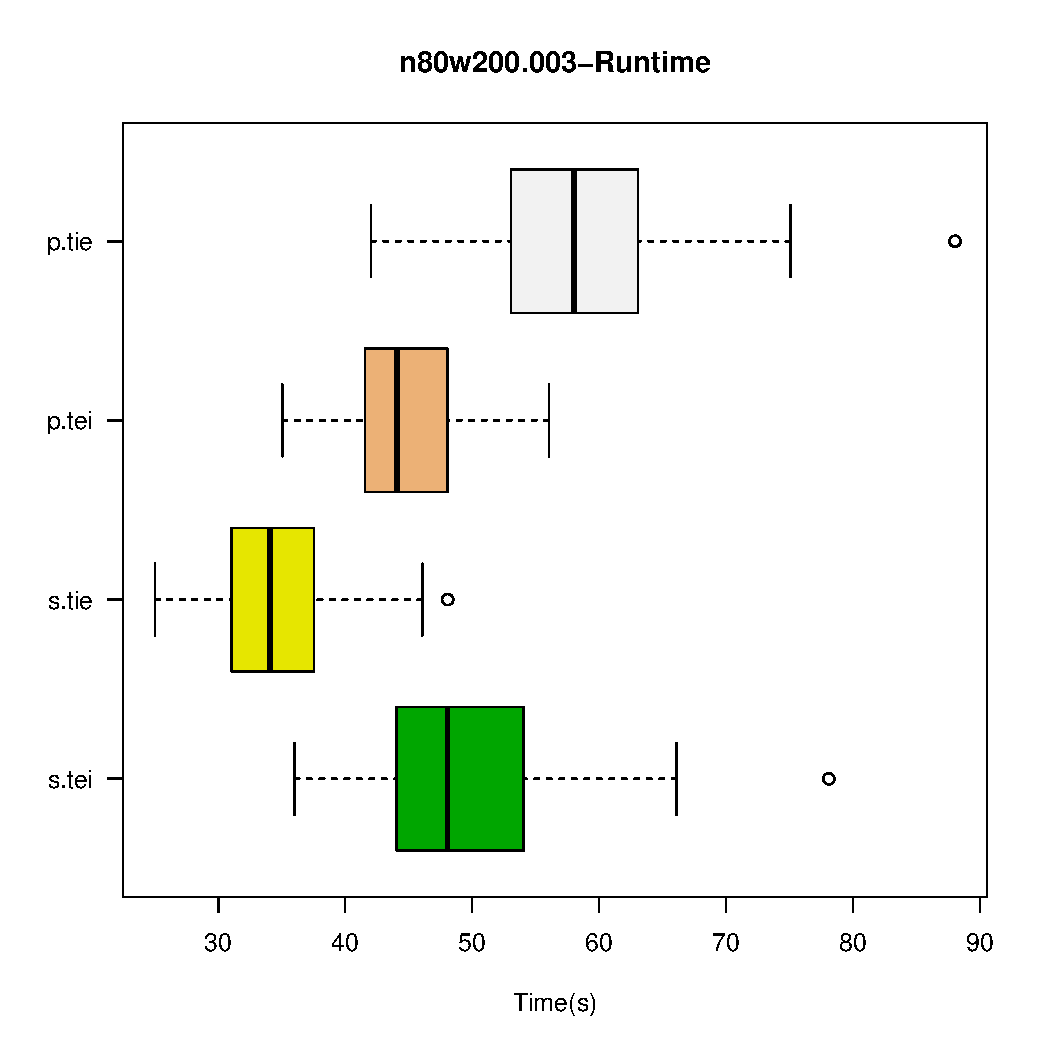
\includegraphics[width=0.6\textwidth,keepaspectratio]{{II/n80w200.003/n80w200.003-CpuTime}.pdf}
\captionof{figure}{n80w200.003 - Runtime boxplots for the different iterative improvement algorithms}
\end{center}

\begin{center}
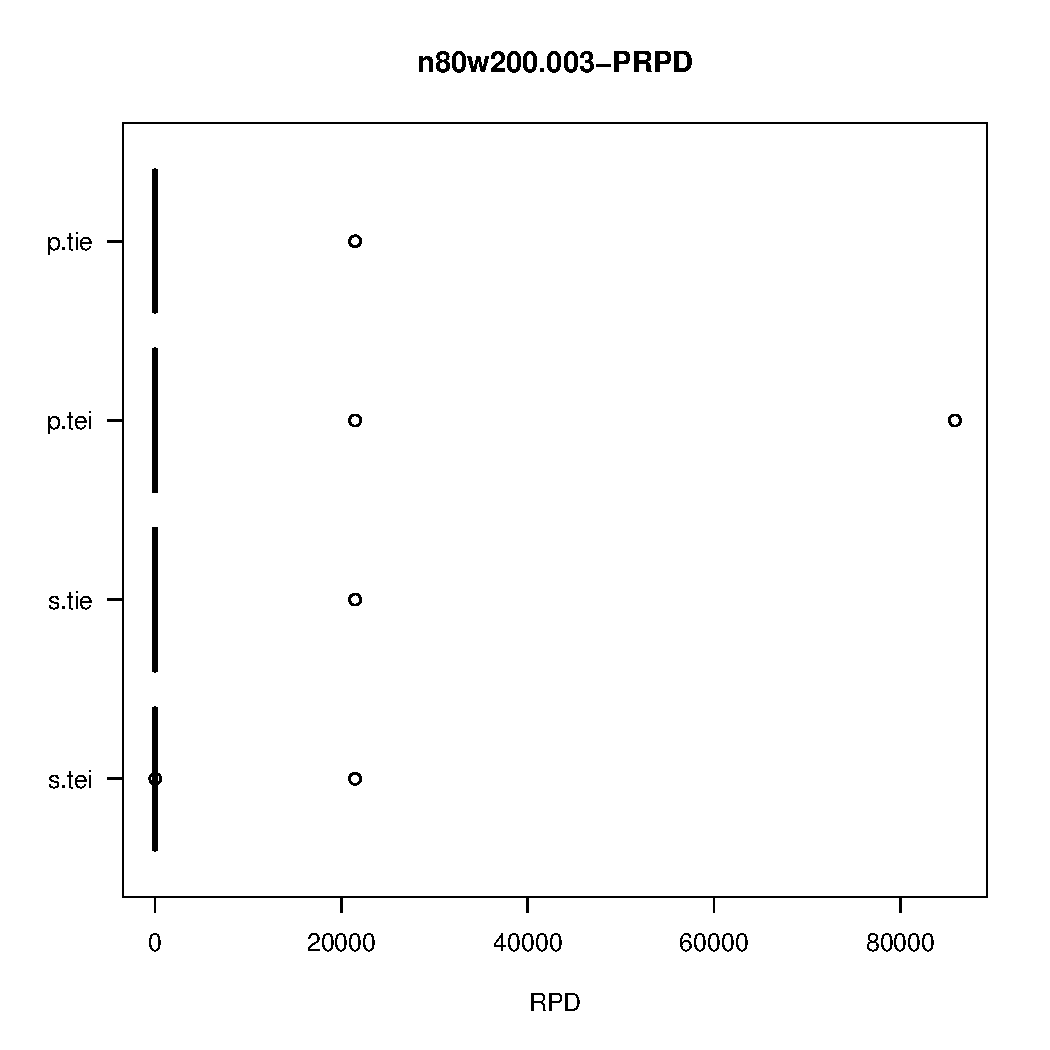
\includegraphics[width=0.6\textwidth,keepaspectratio]{{II/n80w200.003/n80w200.003-PRPD}.pdf}
\captionof{figure}{n80w200.003 - PRPD boxplots for the different iterative improvement algorithms}
\end{center}

\begin{center}
\begin{tabular}{|l|l|}
\hline
\textbf{Test} & \textbf{P-Value} \\
\hline
First vs best - Transpose&4.33123080260219e-18\\
\hline
First vs best - Exchange&7.01070639830382e-18\\
\hline
First vs best - Insert&3.95591160889952e-18\\
\hline
Exchange vs Insert - First&3.95591160889952e-18\\
\hline
Exchange vs Insert - Best&3.95591160889952e-18\\
\hline
\end{tabular}
\captionof{table}{n80w200.003 - Results of Wilcoxon paired signed rank test}
\label{tab:w.8}
\end{center}

\subsubsection{n80w200.004}
\begin{center}
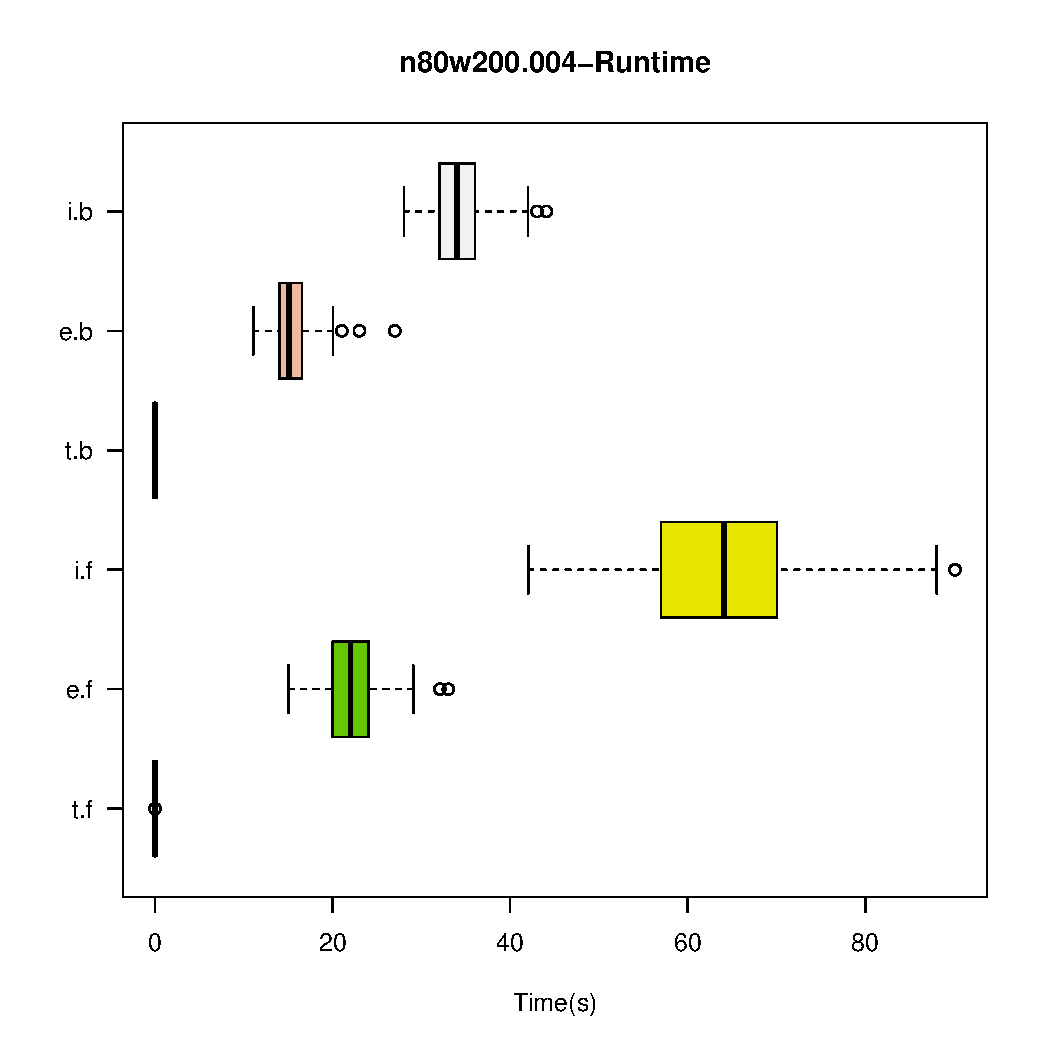
\includegraphics[width=0.6\textwidth,keepaspectratio]{{II/n80w200.004/n80w200.004-CpuTime}.pdf}
\captionof{figure}{n80w200.004 - Runtime boxplots for the different iterative improvement algorithms}
\end{center}

\begin{center}
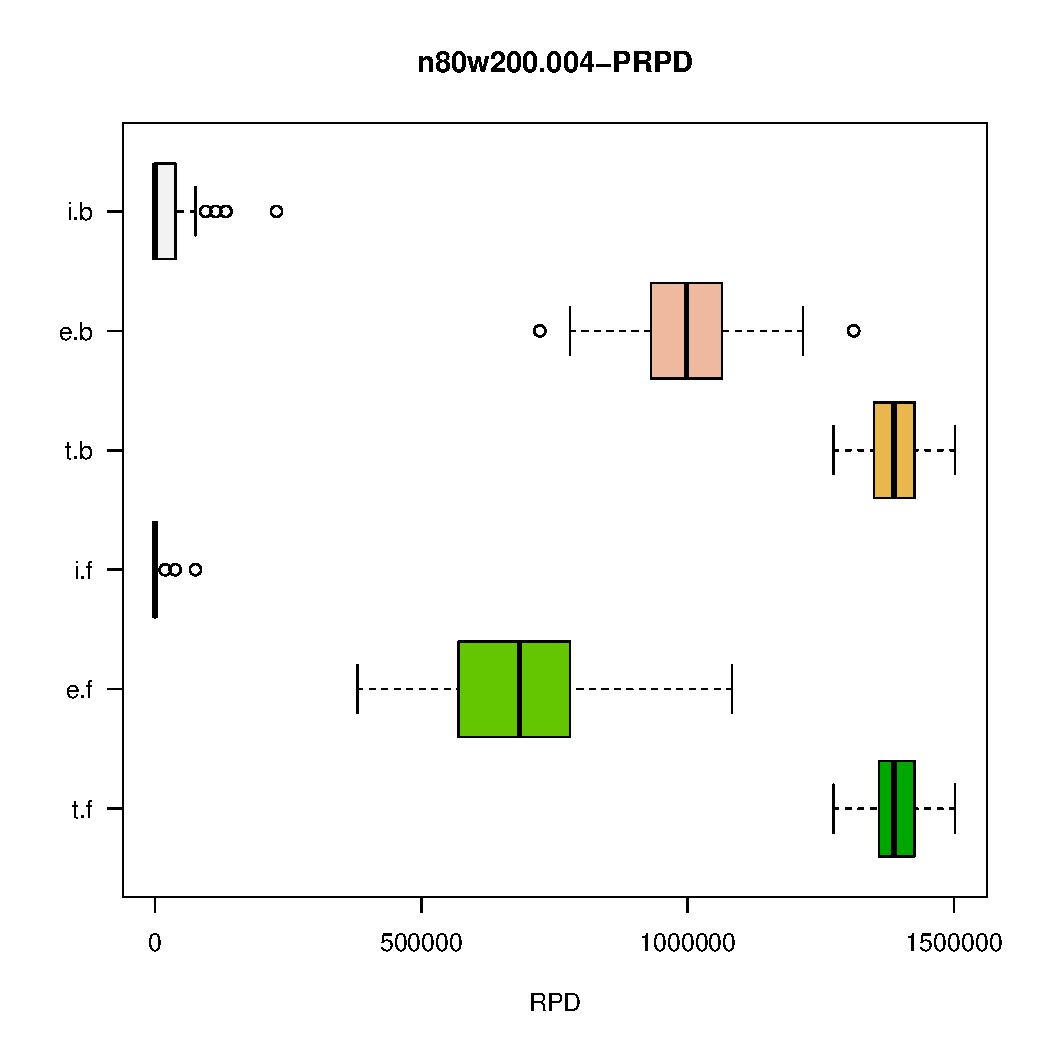
\includegraphics[width=0.6\textwidth,keepaspectratio]{{II/n80w200.004/n80w200.004-PRPD}.pdf}
\captionof{figure}{n80w200.001 - PRPD boxplots for the different iterative improvement algorithms}
\end{center}

\begin{center}
\begin{tabular}{|l|l|}
\hline
\textbf{Test} & \textbf{P-Value} \\
\hline
First vs best - Transpose&4.33123080260219e-18\\
\hline
First vs best - Exchange&2.4473398426105e-17\\
\hline
First vs best - Insert&3.95591160889952e-18\\
\hline
Exchange vs Insert - First&3.95591160889952e-18\\
\hline
Exchange vs Insert - Best&3.95591160889952e-18\\
\hline
\end{tabular}
\captionof{table}{n80w200.004 - Results of Wilcoxon paired signed rank test}
\label{tab:w.9}
\end{center}

\subsubsection{n80w200.005}
\begin{center}
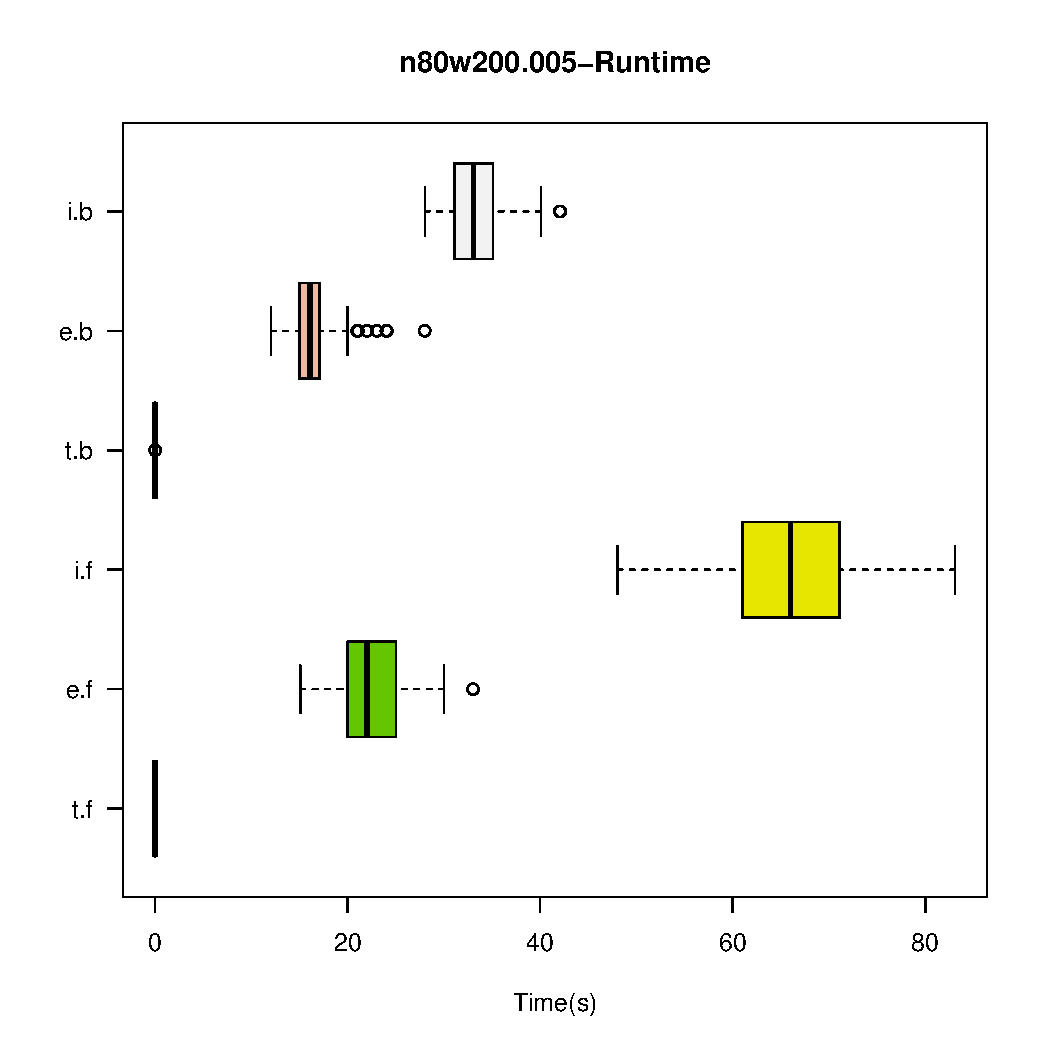
\includegraphics[width=0.6\textwidth,keepaspectratio]{{II/n80w200.005/n80w200.005-CpuTime}.pdf}
\captionof{figure}{n80w200.005 - Runtime boxplots for the different iterative improvement algorithms}
\end{center}

\begin{center}
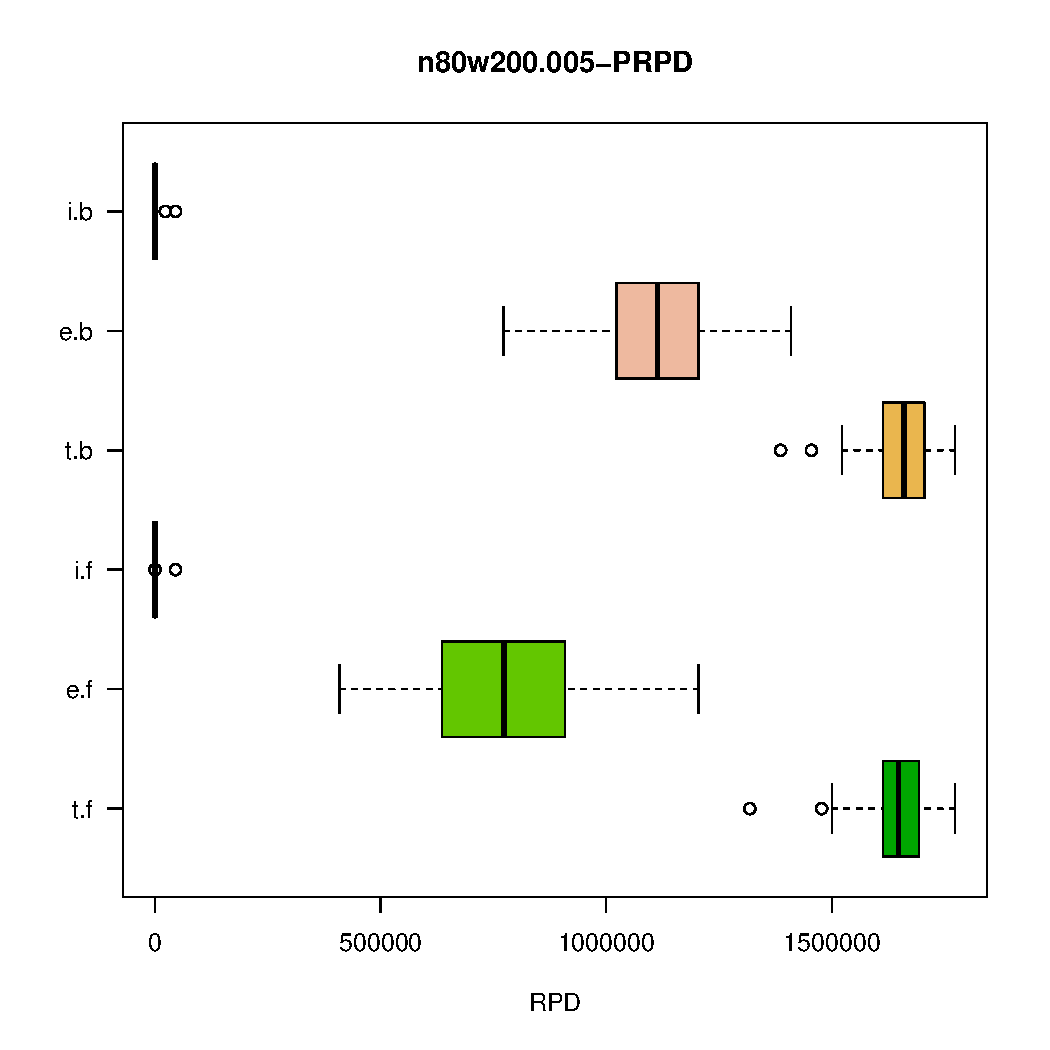
\includegraphics[width=0.6\textwidth,keepaspectratio]{{II/n80w200.005/n80w200.005-PRPD}.pdf}
\captionof{figure}{n80w200.005 - PRPD boxplots for the different iterative improvement algorithms}
\end{center}

\begin{center}
\begin{tabular}{|l|l|}
\hline
\textbf{Test} & \textbf{P-Value} \\
\hline
First vs best - Transpose&4.74166029806301e-18\\
\hline
First vs best - Exchange&1.40854365025687e-16\\
\hline
First vs best - Insert&3.95591160889952e-18\\
\hline
Exchange vs Insert - First&3.95591160889952e-18\\
\hline
Exchange vs Insert - Best&3.95591160889952e-18\\
\hline
\end{tabular}
\captionof{table}{n80w200.005 - Results of Wilcoxon paired signed rank test}
\label{tab:w.10}
\end{center}

\subsection{Statistics}

\subsubsection{Transpose-First Improvement}
\begin{center}
\begin{tabular}{|l|c|l|l|}
\hline
\textbf{Instance}& \textbf{\% Infeasible} & $\mathbf{\bar{PRDP}}$ &$\mathbf{\bar{Runtime}}$\\
\hline
n80w20.001&1&1229712.6&0.0100035563\\
\hline
n80w20.002&1&1028075.17&0.0095843375\\
\hline
n80w20.003&1&1132968.5&0.0098099452\\
\hline
n80w20.005&1&1010681.79&0.0097989762\\
\hline
n80w20.004&1&1226174.6&0.0094877067\\
\hline
n80w200.001&1&1467634.1&0.0098152878\\
\hline
n80w200.002&1&1504523.7&0.0099101404\\
\hline
n80w200.004&1&1388037.6&0.0098893615\\
\hline
n80w200.003&1&1567210.5&0.0097697727\\
\hline
n80w200.005&1&1644110.9&0.0097550971\\
\hline
\end{tabular}
\captionof{table}{Statistics summary for iterative improvement algorithm with Transpose neighborhood and First Improvement pivoting rule}
\label{tab:t.f}
\end{center}

\subsubsection{Transpose-Best Improvement}
\begin{center}
\begin{tabular}{|l|c|l|l|}
\hline
\textbf{Instance}& \textbf{\% Infeasible} & $\mathbf{\bar{PRDP}}$ &$\mathbf{\bar{Runtime}}$\\
\hline
n80w20.001&1&1236039.3&0.014545497\\
\hline
n80w20.002&1&1033090.48&0.0145450422\\
\hline
n80w20.003&1&1137758.7&0.014536776\\
\hline
n80w20.005&1&1014818.46&0.014947609\\
\hline
n80w20.004&1&1232996&0.015151286\\
\hline
n80w200.001&1&1476994.8&0.0147534638\\
\hline
n80w200.002&1&1511281&0.014884921\\
\hline
n80w200.004&1&1392023.3&0.0146445173\\
\hline
n80w200.003&1&1575355.5&0.0143582468\\
\hline
n80w200.005&1&1653419.6&0.0150098656\\
\hline
\end{tabular}
\captionof{table}{Statistics summary for iterative improvement algorithm with Transpose neighborhood and Best Improvement pivoting rule}
\label{tab:t.b}
\end{center}

\subsubsection{Exchange-First Improvement}
\begin{center}
\begin{tabular}{|l|c|l|l|}
\hline
\textbf{Instance}& \textbf{\% Infeasible} & $\mathbf{\bar{PRDP}}$ &$\mathbf{\bar{Runtime}}$\\
\hline
n80w20.001&1&1035718.78&18.390814\\
\hline
n80w20.002&1&884386.3&18.198632\\
\hline
n80w20.003&1&956518.77&18.913801\\
\hline
n80w20.005&1&849054.52&19.043496\\
\hline
n80w20.004&1&1030411.56&19.660314\\
\hline
n80w200.001&1&661322.18&23.117446\\
\hline
n80w200.002&1&813339.6&22.552976\\
\hline
n80w200.004&1&679489.06&22.068859\\
\hline
n80w200.003&1&697450.03&24.338257\\
\hline
n80w200.005&1&760027.65&22.348975\\
\hline
\end{tabular}
\captionof{table}{Statistics summary for iterative improvement algorithm with Exchange neighborhood and First Improvement pivoting rule}
\label{tab:e.f}
\end{center}

\subsubsection{Exchange-Best Improvement}
\begin{center}
\begin{tabular}{|l|c|l|l|}
\hline
\textbf{Instance}& \textbf{\% Infeasible} & $\mathbf{\bar{PRDP}}$ &$\mathbf{\bar{Runtime}}$\\
\hline
n80w20.001&1&1086217.68&13.091453\\
\hline
n80w20.002&1&901762.05&13.365301\\
\hline
n80w20.003&1&1017243.86&13.267128\\
\hline
n80w20.005&1&895720.53&13.5824245\\
\hline
n80w20.004&1&1084080.4&14.189582\\
\hline
n80w200.001&1&1022433.76&16.418229\\
\hline
n80w200.002&1&1075649.94&16.028712\\
\hline
n80w200.004&1&994703.67&15.518766\\
\hline
n80w200.003&1&1094460.9&16.16696\\
\hline
n80w200.005&1&1110949.86&16.566802\\
\hline
\end{tabular}
\captionof{table}{Statistics summary for iterative improvement algorithm with Exchange neighborhood and Best Improvement pivoting rule}
\label{tab:e.b}
\end{center}

\subsubsection{Insert-First Improvement}
\begin{center}
\begin{tabular}{|l|c|l|l|}
\hline
\textbf{Instance}& \textbf{\% Infeasible} & $\mathbf{\bar{PRDP}}$ &$\mathbf{\bar{Runtime}}$\\
\hline
n80w20.001&0.65&16070.27322082&25.88279\\
\hline
n80w20.002&0.83&11803.71462682&28.509938\\
\hline
n80w20.003&0.83&21587.617&28.579453\\
\hline
n80w20.005&0.32&4945.642107&28.672083\\
\hline
n80w20.004&0.49&10894.01867489&28.474429\\
\hline
n80w200.001&0.22&6119.9927045&59.544212\\
\hline
n80w200.002&0&11.2561521&64.580306\\
\hline
n80w200.004&0.11&3049.80805246&63.942238\\
\hline
n80w200.003&0.01&437.87774695&63.687806\\
\hline
n80w200.005&0.01&464.62990671&66.084369\\
\hline
\end{tabular}
\captionof{table}{Statistics summary for iterative improvement algorithm with Insert neighborhood and First Improvement pivoting rule}
\label{tab:i.f}
\end{center}

\subsubsection{Insert-Best Improvement}
\begin{center}
\begin{tabular}{|l|c|l|l|}
\hline
\textbf{Instance}& \textbf{\% Infeasible} & $\mathbf{\bar{PRDP}}$ &$\mathbf{\bar{Runtime}}$\\
\hline
n80w20.001&0.56&14772.44442862&28.769951\\
\hline
n80w20.002&0.84&16009.51797952&30.159812\\
\hline
n80w20.003&0.89&26984.256&30.197019\\
\hline
n80w20.005&0.52&10159.3062354&30.776906\\
\hline
n80w20.004&0.59&18861.32619536&31.013\\
\hline
n80w200.001&0.37&21195.2243605&33.031965\\
\hline
n80w200.002&0&13.2172159&33.011011\\
\hline
n80w200.004&0.42&23019.4946845&34.123681\\
\hline
n80w200.003&0.12&7740.06242146&34.080592\\
\hline
n80w200.005&0.07&2516.0079072&33.450537\\
\hline
\end{tabular}
\captionof{table}{Statistics summary for iterative improvement algorithm with Insert neighborhood and Best Improvement pivoting rule}
\label{tab:i.b}
\end{center}

\subsection{Results discussion}
By looking at tables \ref{tab:t.f}, \ref{tab:t.b}, \ref{tab:e.f}, \ref{tab:e.b} \ref{tab:i.f}, \ref{tab:i.b} on can see that:
\begin{itemize}
\item The neighborhood type has a strong influence on the both the time complexity of the algorithm and the generated solution quality. This is due to the size of the different neighborhoods ($n=80$):
      \begin{itemize}
        \item Transpose - $(n-1)$
        \item Exchange - $\frac{n\cdot(n-1)}{2}$
        \item Insert - $(n-1)^2$
      \end{itemize}
The different size of the neighborhoods corresponds to different degrees of exploration (diversification).
      
\item Transpose and Exchange neighborhoods have smaller runtimes but a percentage of infeasible runs equal to 1. 
Both the algorithm do not allow to find a feasible solution but the Exchange algorithm constructs solutions with a better quality (reduced, but not yet null, constraint violations and total travel time).

\item Insert is the only neighborhood type that allows to generate solutions that are both feasible and closer to the global optima.

\item The first-improvement pivoting rule is generally slower than the best-improvement one, when considering the same neighborhood type.
This is due to the fact that, with the first-improvement pivoting rule, smaller improvement are made to the solution at each iteration, thus requiring and higher number of iteration to converge to a local optima, with respect to the case where the best improvement is chosen at each time step.

\item The quality of the solutions generated using the first-improvement pivoting rule is slightly better thant those generated using the best-improvement one.

\item Tables \ref{tab:w.1}, \ref{tab:w.2}, \ref{tab:w.3}, \ref{tab:w.4}, \ref{tab:w.5}, \ref{tab:w.6}, \ref{tab:w.7}, \ref{tab:w.8}, \ref{tab:w.9}, \ref{tab:w.10} contain, in any case, p-values considerably smaller than the significance level ($\alpha=0.05$). 

This implies that the null hypothesis corresponding to the equality of the median values of the differences of the two distributions can be rejected, hence assessing the existence of a statistically significant difference among the solution quality generated by analyzed algorithms.

\item By looking at the Cpu time, one can easily see that the instances \emph{n80w20.X} have lower runtimes than the \emph{n80w200.X} ones. They can then be considered, with respect to the iterative improvement algorithms, simpler instances with respect to the latter.

\end{itemize}

\end{homeworkProblem}		
